\bartchapterimage{heic0911b.jpg}
\chapter[MAGGIE vs SDSS]{MAGGIE versus SDSS}
\label{cha:MAGGIE_vs_SDSS}
\bartthumb{heic0911b.png}

\minitoc%

\section{Introduction}
\label{sec:vs_introduction}

MAGGIE is designed for an optimal extraction of galaxy groups in several
galaxy surveys such as the SDSS\@. Once the group catalogue in our
possession, we are able to analyze galaxies in both local and global
environments. Our study of environment is motivated by~\cite{Peng+10}
results, showing that with their estimation of the environment of galaxies,
the star formation rate (SFR) is independent of it, except for high mass
galaxies where the SFR is lower in dense environment. But as discussed in
the introduction of the thesis, the tracer used for the environment doesn't
distinguish between both environments. With our results, we make the same
analysis to see modulations with the projected radius in virial units and
the host halo mass.

\section{Data}
\label{sec:data}

\subsection{Stellar masses}
\label{sub:stellar_masses}

We use the galaxy selection and clean up done and provided in
\cite{Tempel+14}. Stellar masses are a principal components of our algorithm
but~\cite{Tempel+14} didn't worked with them, letting us the choice of the
stellar masses to use. In \bartreffigure{stellar_mass_models}, we show that
there are large differences between available models in the SDSS database.
Estimations of some models are different from the other and shouldn't not be
used. A way to deal with this problem is, for each galaxy in the sample, to
use the median of the stellar mass for all models. But sometimes, we don't
have access to the stellar mass of a galaxy and removing it from the sample
will create an supplementary incompleteness. In such situations, we provide
by default the stellar mass estimation based on~\cite{Bell+03}. Those
fitting formulas allows to get the stellar mass of a galaxy with only
informations about its colour and luminosity. Several colors are available
to make the computation. We show in \bartreffigure{bell_comparison} the
stellar mass distribution for several colors used on the formulas
of~\cite{Bell+03}. The $r-z$ color seems to create less outliers in stellar
masses than other bands. A possible explanation is that the magnitude bands
involved in the computation are less sensitive to the dust extinction and
thus provide an accurate estimation of the stellar mass. So, we use only the
stellar mass from $r-z$ color for galaxies without models in the SDSS
database.

\begin{figure}[htb]
    \centering
    \begin{minipage}{0.49\linewidth}
        \centering
        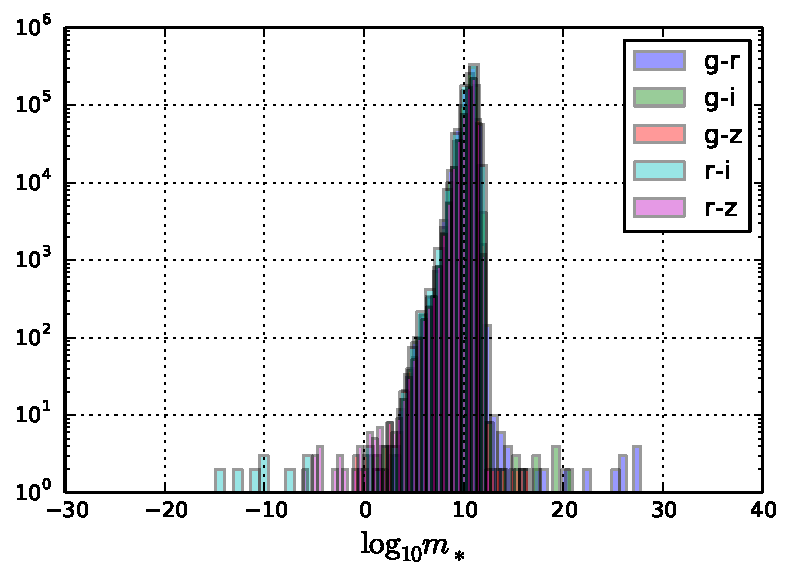
\includegraphics[width=\linewidth]{%
            figures/maggie_vs_sdss/bell_stellar_masses.pdf%
        }
        \captionof{figure}{The distribution of stellar masses in solar units
            for galaxies on the SDSS with the median of models described in
            \bartreffigure{stellar_mass_models} and the default value for
            galaxies without stellar mass estimations from~\cite{Bell+03}
            for different magnitude colors. The number of non-physical
        values for stellar masses is reduced by using the $r-z$ color, less
    affected by dust extinction and so more
accurate.\label{fig:bell_comparison}}
    \end{minipage}
    \begin{minipage}{0.49\linewidth}
        \centering
        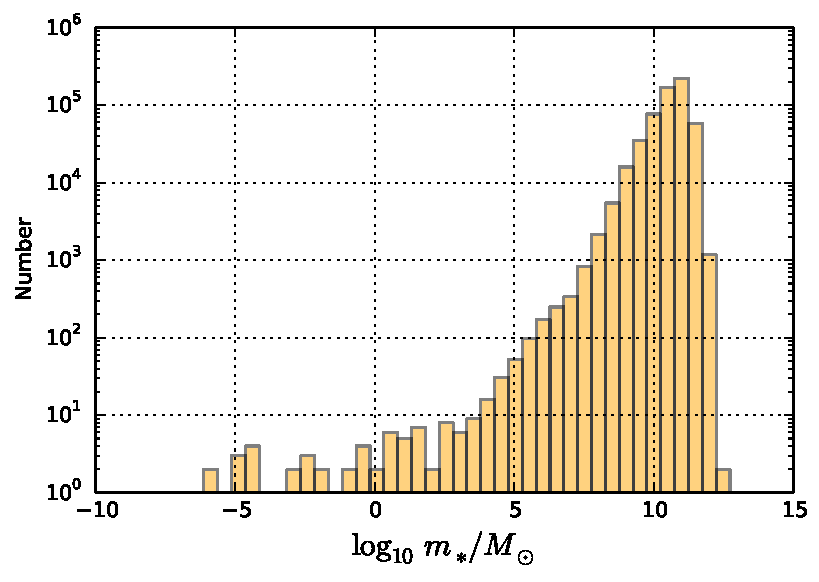
\includegraphics[width=\linewidth]{%
            figures/maggie_vs_sdss/sdss_stellar_masses_final.pdf%
        }
        \captionof{figure}{The distribution of stellar masses in solar units
            for our SDSS galaxy sample once chosen the $r-z$ color magnitude
            as default estimation. There is no high mass galaxies, but some
            stellar masses are still with bad low values. We keep them to
            avoid introducing an supplementary incompleteness in the galaxy
            sample.\label{fig:stellar_mass_distribution}}
    \end{minipage}
\end{figure}

The resulting stellar mass distribution from our galaxy sample is shown in
\bartreffigure{stellar_mass_distribution}. No galaxies have too high stellar
masses, but a lot of them are very low and seems to not be physical. But we
can't remove them without introducing an incompleteness so we keep them as
it in the sample.

\subsection{Star formation rate}
\label{sub:star_formation_rate}

Measures of the star formation rate suffers the same problems as stellar
masses: too many models that not necessarily agree on the estimation. The
same analysis of comparison of the SFR measures is shown on
\bartreffigure{sfr_comparison}. Some models disappeared such as PCAWiscM11
and PCAWiscBC03 not providing SFR estimation for galaxies, PassivePort and
StarFormingPort having too many galaxies with null SFR\@. MPA-JHU has
several estimations of the SFR\@: one based only on informations acquired by
the fiber pointing to the galaxy to get its spectrum (suffixed by
\emph{fib}) and the other where an extrapolation of the informations is done
outside the aperture (suffixed by \emph{tot}).

\begin{figure}[htb]
    \centering
    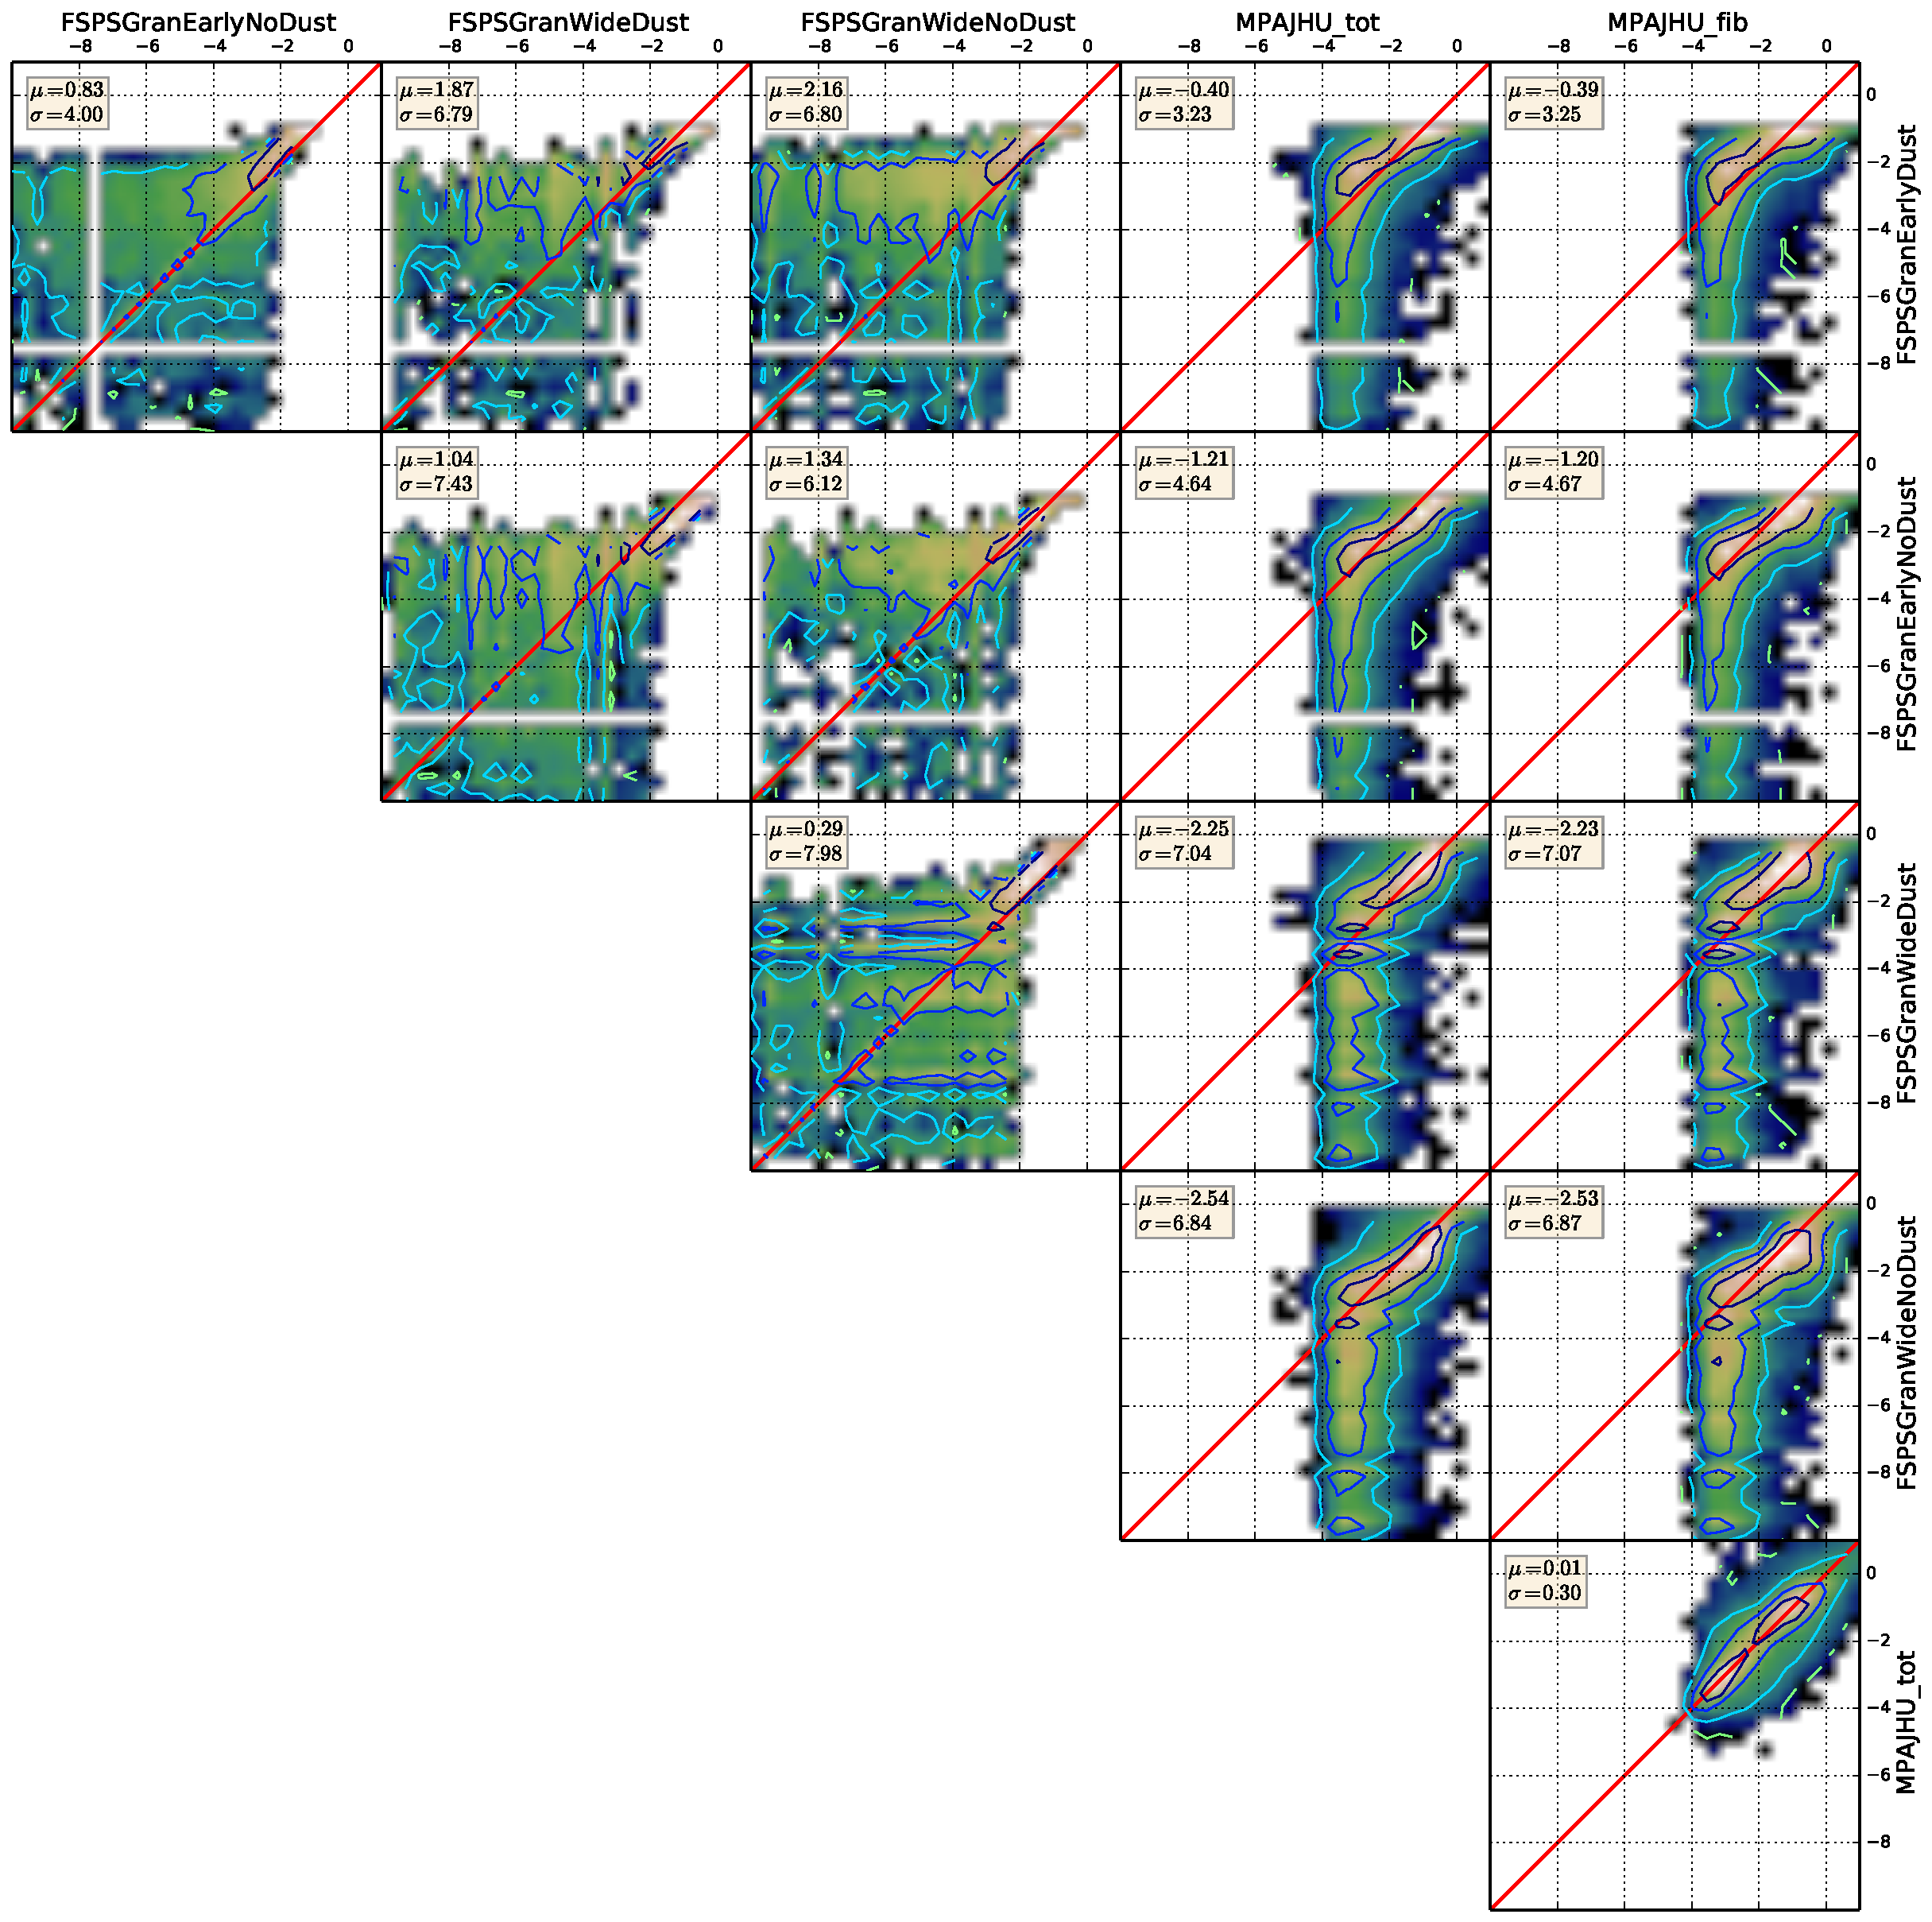
\includegraphics[width=\linewidth]{%
        figures/maggie_vs_sdss/ssfr_models.pdf%
    }
    \caption{Comparison of several specific star formation rate (SFR)
        measures from different models. FSPSGranWideDust,
        FSPSGranWideNoDust, FSPSGranEarlyDust and FSPSGranEarlyNoDust
        from~\cite{Conroy+09} and MPA-JHU~\cite{Brinchmann+04, Kauffmann+03,
        Tremonti+04}. Two variants exist for MPA-JHU according to if the
        estimation is based on the region of the fiber (suffixed \emph{fib})
        or is also extrapolated (suffixed \emph{tot}). Axes are $\log_{10}
        SSFR$ in units of $\mathrm{Gyr}^{-1}$. We show also the bias and
        dispersion of the log-difference of models. FSPS models are not very
        consistent between each other and we don't use them. MPA-JHU are
        relatively coherent but we should prefer the \emph{total} estimation
    since with the fiber estimation not all the stellar population of the
galaxy is probed.\label{fig:sfr_comparison}}
\end{figure}

As we can see, FSPS are not coherent between them and since it will
introduce too many galaxies with a bad estimation of the SSFR, we don't use
them in our analysis. Bias and scatter between both models of MPA-JHU are
small, making them model a good choice for a measure of the star formation
on galaxies. Our preference goes to the \emph{total} model, since when the
entire stellar population of the galaxy can't be accessed by the fiber, the
extrapolation allows a better estimation of the stellar mass and SFR\@.

\begin{figure}[htb]
    \centering
    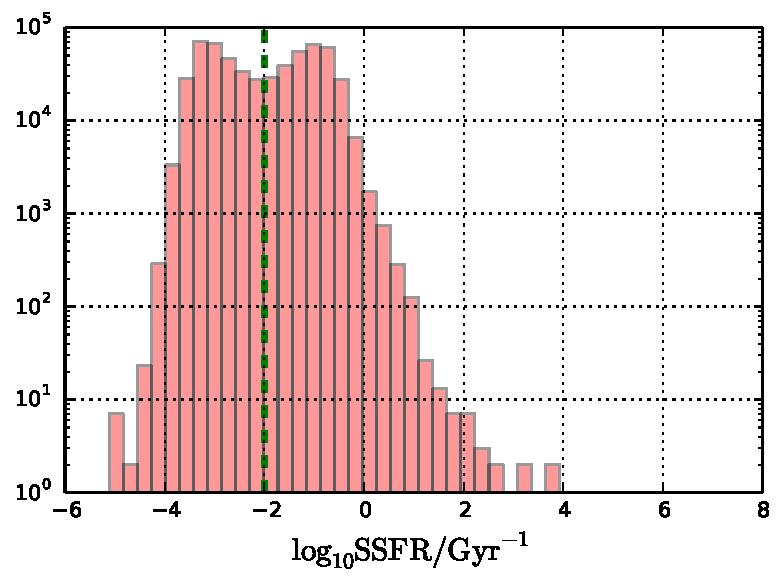
\includegraphics[width=0.8\linewidth]{%
        figures/maggie_vs_sdss/sfr_distribution.pdf%
    }
    \caption{The distribution of SSFR from the MPA-JHU model. We can see a
    bi-modality in the distribution, splitting galaxies into star forming
and passive galaxies (the \emph{green dashed} line shows the
separation).\label{fig:ssfr_distribution}}
\end{figure}

The resulting distribution of the SSFR in \bartreffigure{ssfr_distribution}
shows that galaxies can be classified on two categories: a star forming
population where an important fraction of the galaxy stellar mass is
produced in a time scale of $1$ Gyr and a passive one, where the star
formation represents a low part of its stellar mass. The green line in
\bartreffigure{ssfr_distribution} shows this limit. It will be useful when
searching if there is a modulation with the environment of the fraction of
young galaxies.

\section{Environment modulation}
\label{sec:environment_modulation}

\cite{Peng+10} has shown that the mean SSFR is not very dependent of the
environment, using the over-density as a tracer. But we can go further and
see its modulation with local and global environment through the projected
radius of the galaxy in its halo and the virial mass of the host halo.

We tried this with both MAGGIE and the group catalogues provided
by~\cite{Tempel+14} for a simple comparison.

\subsection{MAGGIE}
\label{sub:ssfr_maggie}

We use two complete catalogues to show this modulation: catalogue 3 too have
sufficient statistics in number of galaxies and catalogue 5 to see the
behaviour at larger redshifts.

\begin{figure}[htb]
    \centering
    \begin{minipage}{\linewidth}
        \centering
        \begin{minipage}{\linewidth}
            \centering
            \subfloat[Catalogue 3]{%
                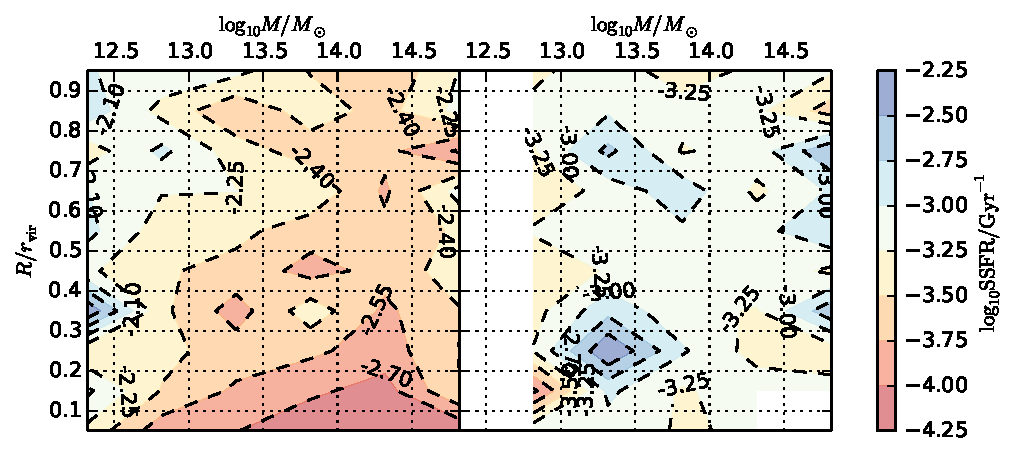
\includegraphics[height=0.2\textheight]{%
                    {figures/maggie_vs_sdss/sdss.0.mean_ssfr_2}.pdf%
                }
            }
        \end{minipage}
        \begin{minipage}{\linewidth}
            \centering
            \subfloat[Catalogue 5]{%
                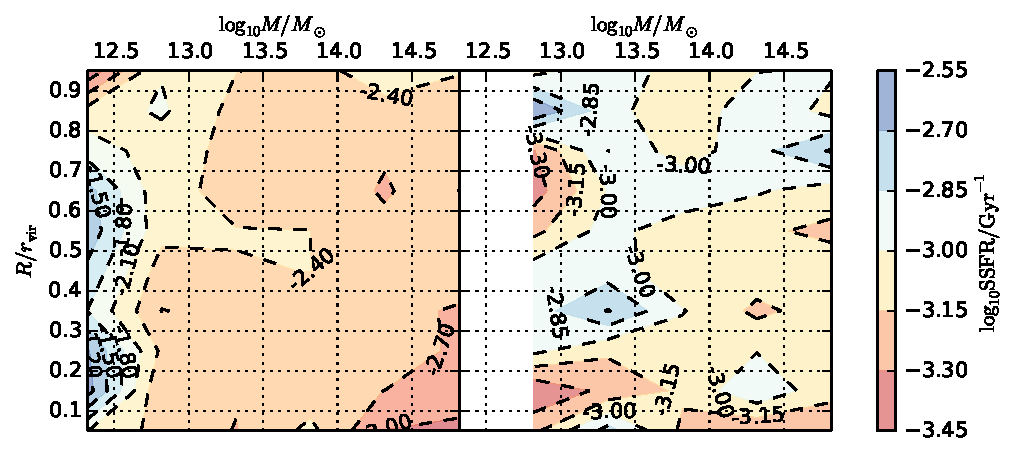
\includegraphics[height=0.2\textheight]{%
                    {figures/maggie_vs_sdss/sdss.0.mean_ssfr_4}.pdf%
                }
            }
        \end{minipage}
        \captionof{figure}{Mean SSFR for galaxies with
            $10\leqslant\log_{10}m_*<11$ (left panel) and
            $11\leqslant\log_{10}m_*<12$ in function of the projected radius
            in units of virial radius (local environment) and of the virial
            mass in solar units (global environment), for galaxy groups
        found with MAGGIE.\label{fig:ssfr_mean}}
    \end{minipage}
    \begin{minipage}{\linewidth}
        \centering
        \begin{minipage}{\linewidth}
            \centering
            \subfloat[Catalogue 3]{%
                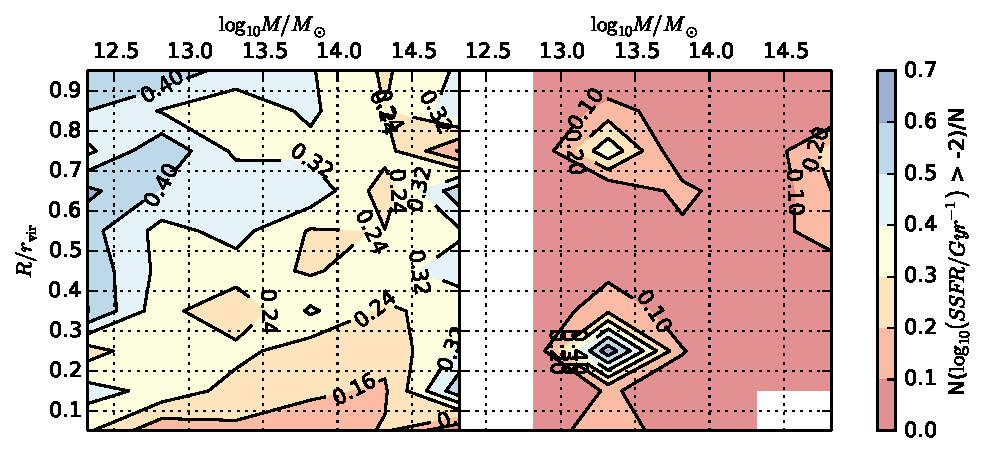
\includegraphics[height=0.2\textheight]{%
                    {figures/maggie_vs_sdss/sdss.0.fraction_over_minus_2_2}.pdf%
                }
            }
        \end{minipage}
        \begin{minipage}{\linewidth}
            \centering
            \subfloat[Catalogue 5]{%
                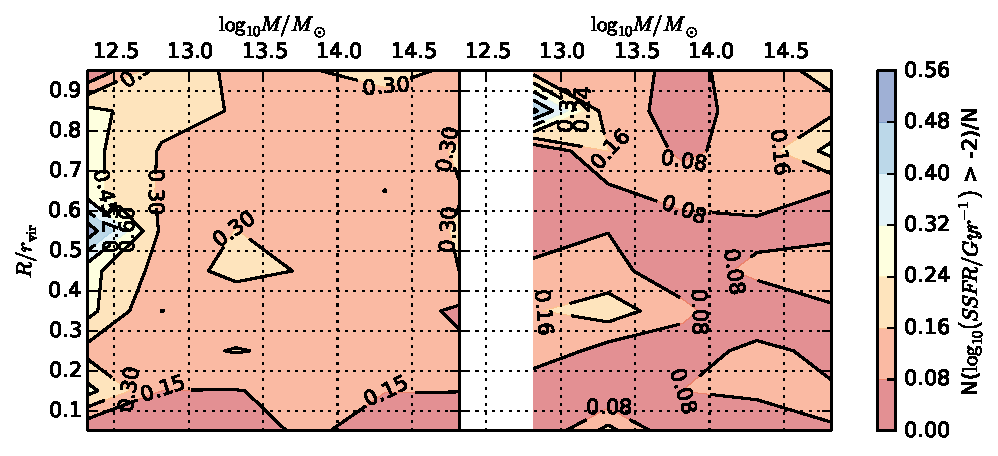
\includegraphics[height=0.2\textheight]{%
                    {figures/maggie_vs_sdss/sdss.0.fraction_over_minus_2_4}.pdf%
                }
            }
        \end{minipage}
        \captionof{figure}{Fraction of galaxies classified as star forming
        galaxies according the criterion of
    \bartrefsubsection{star_formation_rate} for the same range in stellar
masses as in \bartreffigure{ssfr_mean}, with galaxy group from
MAGGIE.\label{fig:ssfr_fraction}}
    \end{minipage}
\end{figure}

\begin{figure}[htb]
    \centering
    \begin{minipage}{\linewidth}
        \centering
        \begin{minipage}{\linewidth}
            \centering
            \subfloat[Catalogue 3]{%
                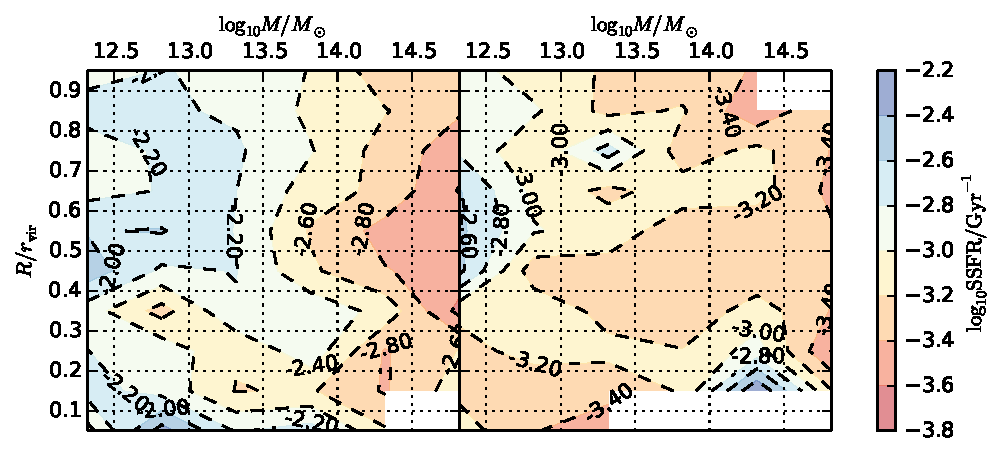
\includegraphics[height=0.2\textheight]{%
                    {figures/maggie_vs_sdss/tempel.0.mean_ssfr_2}.pdf%
                }
            }
        \end{minipage}
        \begin{minipage}{\linewidth}
            \centering
            \subfloat[Catalogue 5]{%
                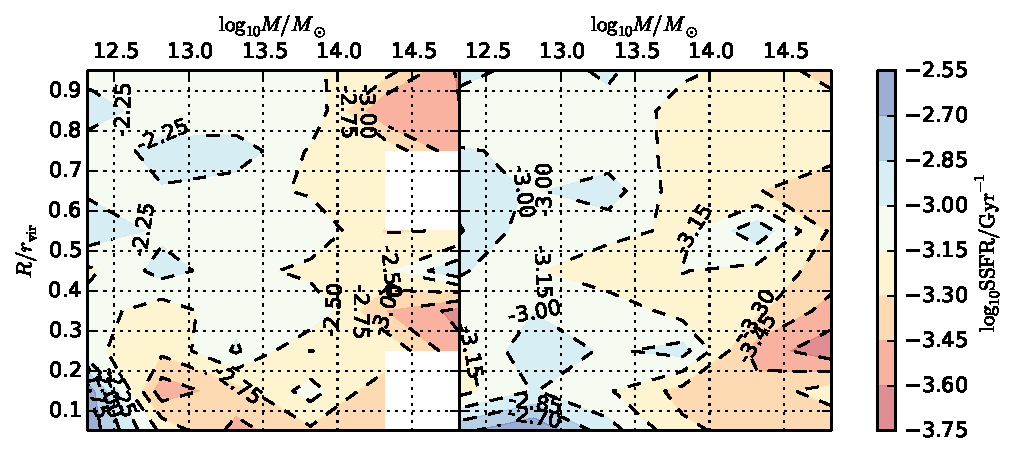
\includegraphics[height=0.2\textheight]{%
                    {figures/maggie_vs_sdss/tempel.0.mean_ssfr_4}.pdf%
                }
            }
        \end{minipage}
        \captionof{figure}{Same as \bartreffigure{ssfr_mean} but for galaxy
        groups from~\cite{Tempel+14}.\label{fig:ssfr_mean_tempel}}
    \end{minipage}
    \begin{minipage}{\linewidth}
        \centering
        \begin{minipage}{\linewidth}
            \centering
            \subfloat[Catalogue 3]{%
                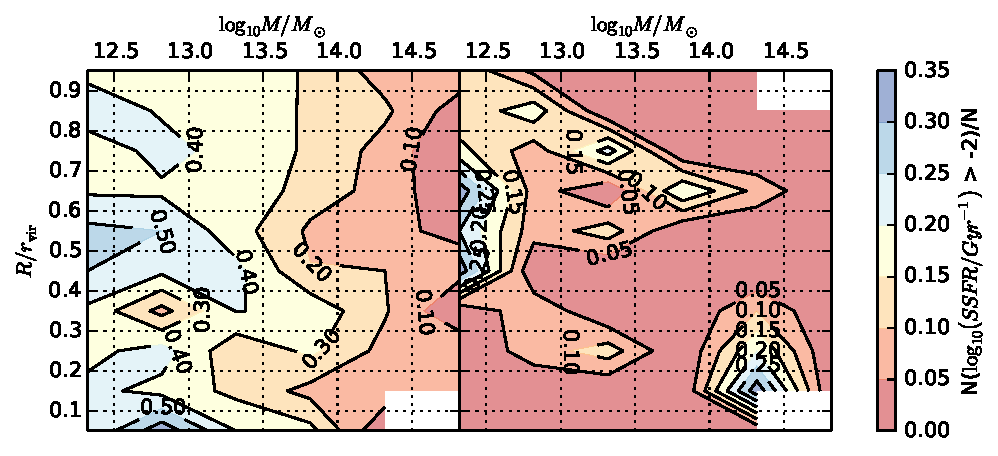
\includegraphics[height=0.2\textheight]{%
                    {figures/maggie_vs_sdss/tempel.0.fraction_over_minus_2_2}.pdf%
                }
            }
        \end{minipage}
        \begin{minipage}{\linewidth}
            \centering
            \subfloat[Catalogue 5]{%
                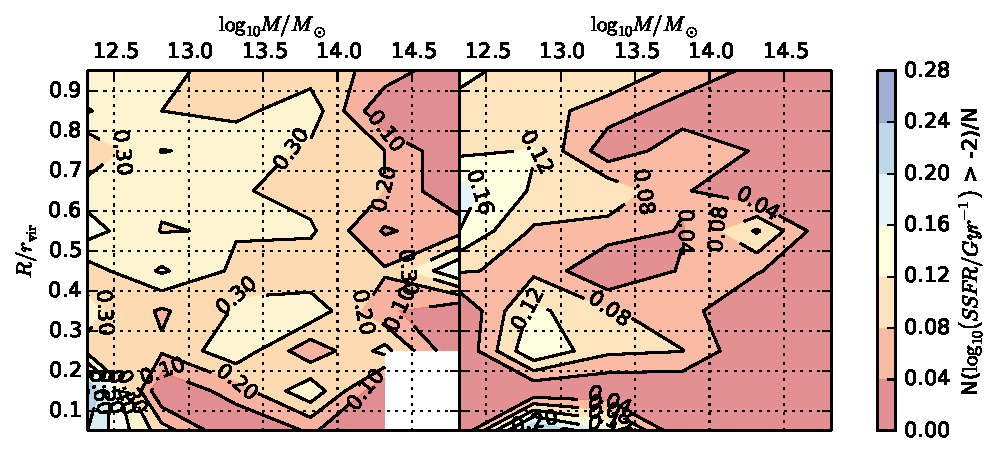
\includegraphics[height=0.2\textheight]{%
                    {figures/maggie_vs_sdss/tempel.0.fraction_over_minus_2_4}.pdf%
                }
            }
        \end{minipage}
        \captionof{figure}{Same as \bartreffigure{ssfr_fraction} but for
        galaxy groups
    from~\cite{Tempel+14}.\label{fig:ssfr_fraction_tempel}}
    \end{minipage}
\end{figure}
